\section{Model Architecture Design}

To achieve deterministic results and reproducibility, the random seed \textbf{42} is set at the beginning of each script. This ensures that the same random initialization is used for each run, leading to consistent results across different experiments:

\begin{minipage}{0.9\linewidth}\begin{lstlisting}[caption={Settings to achieve deterministic results and reproducibility.},label={lst:deterministic-results}]
RANDOM_SEED = 42

seed(RANDOM_SEED)
np.random.seed(RANDOM_SEED)

torch.manual_seed(RANDOM_SEED)
torch.cuda.manual_seed_all(RANDOM_SEED)

torch.backends.cudnn.deterministic = True
torch.backends.cudnn.benchmark = False
\end{lstlisting}\end{minipage}

The random seed is set for the Python, NumPy and PyTorch random number generator. Additionally, the CuDNN backend is set to deterministic mode to ensure that the results are reproducible on the GPU.

\subsection{Guessing Baseline}

As a starting point and to get familiar with the dataset and the Kaggle competition, a simple guessing baseline is implemented. The baseline assigns the most frequent class label to all test samples. This approach provides a lower bound on model performance and serves as a reference point for evaluating the effectiveness of more sophisticated models. The head of the submission file (`submission-0.14105\_Loose-Silky-bent.csv`) is shown below:

\begin{minipage}{0.9\linewidth}\begin{lstlisting}[language={},caption={Guessing baseline submission file.},label={lst:guessing-baseline}]
file,species
1b490196c.png,Loose Silky-bent
85431c075.png,Loose Silky-bent
506347cfe.png,Loose Silky-bent
7f46a71db.png,Loose Silky-bent
668c1007c.png,Loose Silky-bent
...
\end{lstlisting}\end{minipage}

In this case, all \textbf{794} test samples are assigned the class label ``Loose Silky-bent'', which is the most frequent class in the training dataset. The F1-score of this baseline is \textbf{0.14105}.

\subsection{Custom CNN}

The custom CNN architecture is designed to capture features relevant to seedling classification, while being lightweight enough to be effectively trained locally on the given dataset. The model consists of a series of convolutional and pooling layers followed by fully connected layers to learn hierarchical features and make class predictions.

\begin{figure}[htbp]
    \centerline{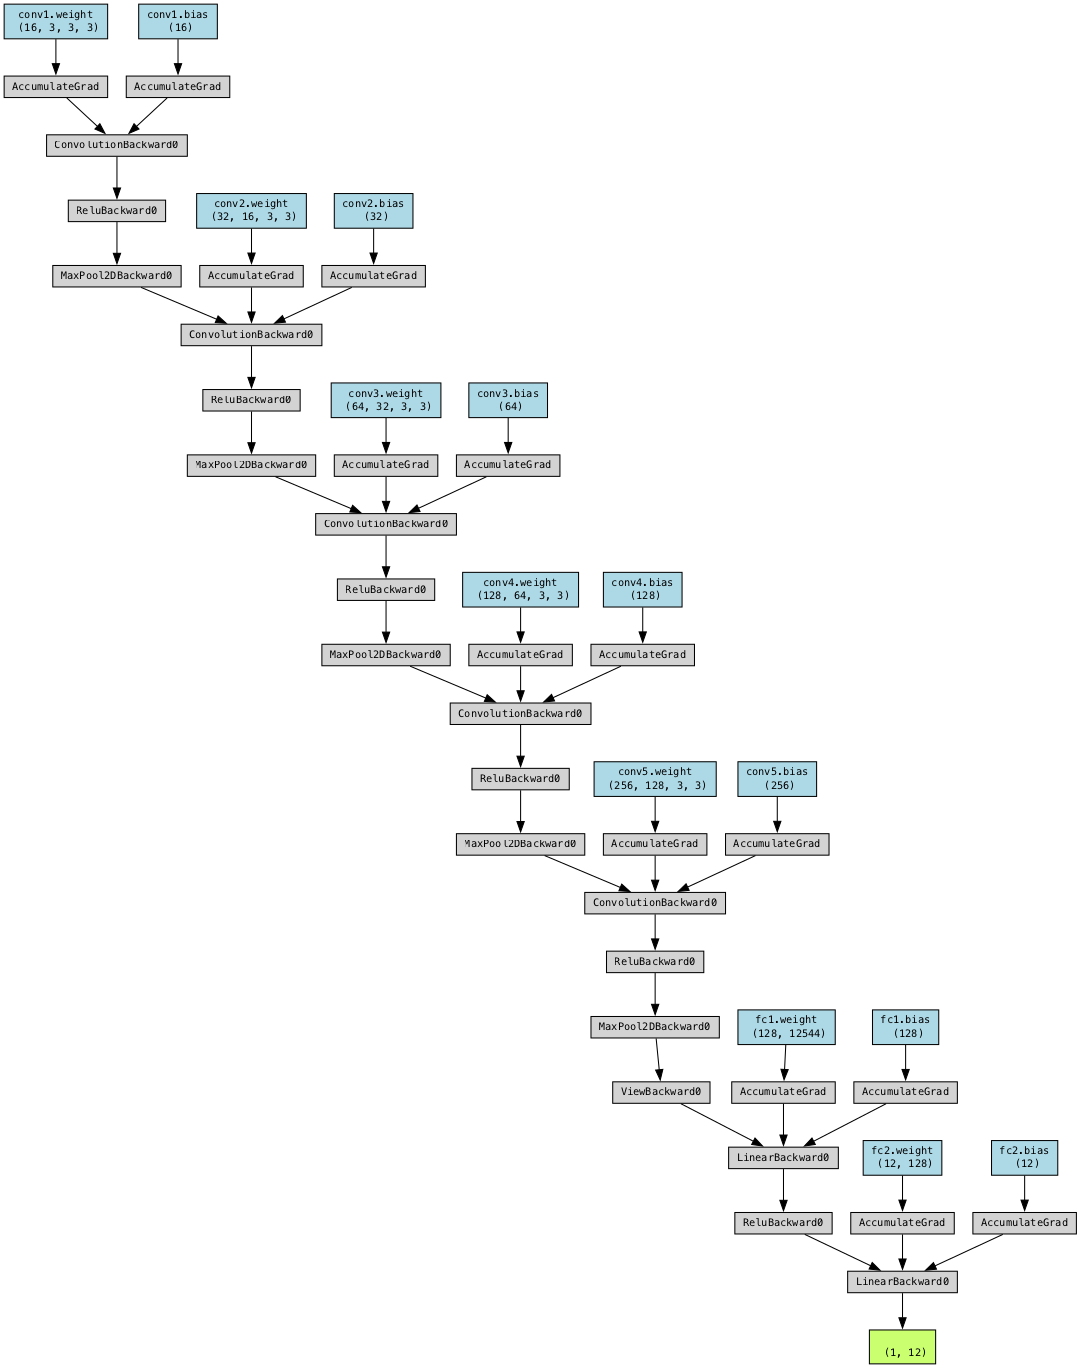
\includegraphics[width=0.9\linewidth]{../../resources/custom_cnn/architecture.png}}
    \caption{Custom CNN Architecture}
    \label{fig:custom-cnn-architecture}
\end{figure}

As shown in \ref{fig:custom-cnn-architecture}, the network begins with a series of convolutional layers, with the number of filters gradually increasing from 16 to 256. These convolutional layers, each followed by a Rectified Linear Unit (ReLU) activation, extract spatial features such as edges, textures and patterns from the images. To reduce spatial dimensions and computational complexity, max-pooling layers are applied after each convolutional block to focus on the most salient features.

After the convolutional and pooling stages, the feature maps are flattened into a 1D vector that serves as the input to the fully connected layers. The first fully connected layer has 128 units and captures high-level abstract features, while the final fully connected layer maps these features to the 12 target classes, producing the class probabilities.

\begin{minipage}{0.9\linewidth}\begin{lstlisting}[language={},caption={Custom CNN model summary.},label={lst:custom-cnn-summary}]
================================
Total params: 1,999,916
Trainable params: 1,999,916
Non-trainable params: 0
--------------------------------
Input size (MB): 0.57
Forward/backward pass size (MB): 26.70
Params size (MB): 7.63
Estimated Total Size (MB): 34.91
--------------------------------
\end{lstlisting}\end{minipage}

The final custom CNN model has approximately \textbf{2 million} parameters, making it lightweight and computationally efficient. The model architecture is designed to capture relevant features for seedling classification while being suitable for training on a moderate-sized dataset.

\subsection{Pre-trained CNN}

As an alternative to training a custom CNN from scratch, a pre-trained CNN can be used to leverage learned features from a large dataset. The pre-trained model ResNet-18 \cite{DBLP:journals/corr/HeZRS15} is used as a feature extractor, where the final classification layer is replaced with a new fully connected layer to predict the 12 plant seedling classes:

\begin{minipage}{0.9\linewidth}\begin{lstlisting}[caption={Replacing the final classification layer of a pre-trained ResNet-18 model.},label={lst:pre-trained-cnn}]
from torchvision import models
from torch.nn import Linear

model = models.resnet18(
    weights=models.ResNet18_Weights.DEFAULT
)
model.fc = Linear(
    in_features=model.fc.in_features,
    out_features=len(dataset.classes),
)
\end{lstlisting}\end{minipage}

The ResNet-18 model is pre-trained on the ImageNet dataset \cite{5206848ImageNet} and has shown strong performance on a variety of computer vision tasks. By using a pre-trained model, the network can leverage the learned features from ImageNet to improve performance on the plant seedlings dataset. The final classification layer is replaced to adapt the model to the specific classification task.

\begin{minipage}{0.9\linewidth}\begin{lstlisting}[language={},caption={Pre-trained CNN model summary.},label={lst:pre-trained-cnn-summary}]
================================
Total params: 11,182,668
Trainable params: 11,182,668
Non-trainable params: 0
--------------------------------
Input size (MB): 0.57
Forward/backward pass size (MB): 62.79
Params size (MB): 42.66
Estimated Total Size (MB): 106.02
--------------------------------
\end{lstlisting}\end{minipage}

This pre-trained CNN model has approximately \textbf{11 million} parameters, making it more complex than the custom CNN. However, the pre-trained weights allow the model to learn more robust features and hopefully achieve better performance on the plant seedlings dataset.

\subsection{Pre-trained ViT}

Another approach is to use a ViT \cite{DBLP:journals/corr/abs-2010-11929} as the backbone architecture. The ViT model is pre-trained on a large-scale dataset and then fine-tuned on the plant seedlings dataset. The final classification head is replaced with a new linear layer to predict the 12 plant seedling classes:

\begin{minipage}{0.9\linewidth}\begin{lstlisting}[caption={Replacing the final classification layer of a pre-trained ViT model.},label={lst:pre-trained-vit}]
import timm
import torch

model = timm.create_model(
    "vit_base_patch16_224",
    pretrained=True,
    num_classes=num_classes
)
model.head = torch.nn.Linear(
    model.head.in_features,
    num_classes
)
\end{lstlisting}\end{minipage}

Instead of fine-tuning the entire model, the pre-trained weights of the `vit\_base\_patch16\_224` model \cite{Wightman_PyTorch_Image_Models} are frozen, and only the classification head is trained on the plant seedlings dataset. This approach leverages the powerful feature extraction capabilities of the pre-trained model while adapting the final layer to the specific classification task. Furthermore the computational cost is reduced compared to training the entire model from scratch or fine-tuning all layers:

\begin{minipage}{0.9\linewidth}\begin{lstlisting}[caption={Freezing the pre-trained ViT backbone and training only the classification head.},label={lst:freeze-vit-backbone}]
for param in model.parameters():
    param.requires_grad = False

for param in model.head.parameters():
    param.requires_grad = True
\end{lstlisting}\end{minipage}

\begin{minipage}{0.9\linewidth}\begin{lstlisting}[language={},caption={Pre-trained ViT model summary.},label={lst:pre-trained-vit-summary}]
================================
Total params: 85,655,820
Trainable params: 9,228
Non-trainable params: 85,646,592
--------------------------------
Input size (MB): 0.57
Forward/backward pass size (MB): 479.03
Params size (MB): 326.75
Estimated Total Size (MB): 806.35
--------------------------------
\end{lstlisting}\end{minipage}

The ViT model has approximately \textbf{85 million} parameters, but only \textbf{9,228} of them are trainable. This makes the model computationally efficient while still benefiting from the powerful feature extraction capabilities of the pre-trained ViT model.

\subsection{Ensemble}

A final ensemble is created by combining the predictions of all three models (custom CNN, pre-trained CNN, pre-trained ViT) using a simple weighted average. The weights are determined based on the performance of each model on the test set:

\begin{minipage}{0.9\linewidth}\begin{lstlisting}[caption={Ensemble predictions using a weighted average.},label={lst:ensemble}]
import torch.nn.functional as F

model_custom_cnn.eval()
model_resnet.eval()
model_vit.eval()

w_custom_cnn = 0.25
w_resnet = 0.25
w_vit = 1 - w_custom_cnn - w_resnet

with torch.no_grad():
    for images, image_names in test_loader:
        ...

        probs_custom_cnn = F.softmax(model_custom_cnn(images), dim=1)
        probs_resnet = F.softmax(model_resnet(images), dim=1)
        probs_vit = F.softmax(model_vit(images), dim=1)

        probs_ensemble = w_custom_cnn * probs_custom_cnn + w_resnet * probs_resnet + w_vit * probs_vit

        _, preds = torch.max(probs_ensemble, 1)
\end{lstlisting}\end{minipage}

The ensemble combines the strengths of each individual model to improve overall performance and robustness. By averaging the predictions of multiple models, the ensemble can reduce the impact of individual model weaknesses and provide more reliable predictions. As the ViT model achieved the highest performance on the test set, it is assigned the highest weight in the ensemble (0.5), while the custom CNN and ResNet models are assigned equal weights (both 0.25).